\documentclass[a4paper,titlepage]{report}

\usepackage[utf8]{inputenc}
\usepackage{graphicx}
\usepackage[a4paper, margin=1in]{geometry}
\usepackage{titlesec}
\usepackage[dvipsnames]{xcolor}
\usepackage{amsmath}
\usepackage{booktabs}
\usepackage{cellspace}
\usepackage{tabularx}
\usepackage{caption}
\usepackage{calc}
\usepackage{ragged2e}
\usepackage{multirow}
\usepackage{hyperref} % Per i link nell'indice
\usepackage{tocbibind} % Per includere l'indice nel sommario
\usepackage{tikz}
\usepackage{listings}
\usepackage{mdframed}
\usepackage[utf8]{inputenc} % This allows UTF-8 encoding
\usepackage[T1]{fontenc} % This ensures that fonts support special characters

\setlength\cellspacetoplimit{5pt}
\setlength\cellspacebottomlimit{4pt}

\definecolor{myBlue}{rgb}{0.0745, 0.2157, 0.4118}
\definecolor{myLightBlue}{rgb}{0, 0.5647, 0.5843}
\definecolor{numb}{RGB}{255,0,0}
\definecolor{punct}{RGB}{0,0,255}
\definecolor{delim}{RGB}{20,105,176}
\definecolor{comment}{RGB}{0,128,0}
\definecolor{string}{RGB}{163,21,21}
\definecolor{keyword}{RGB}{0,0,255}

\titleformat{\section}[hang]{\Large\bfseries\color{myBlue}}{}{0px}{}[\titlerule]
\titleformat{\subsection}[hang]{\large\bfseries\color{myLightBlue}}{}{0em}{}
\titleformat{\subsubsection}[hang]{\bfseries\color{myBlue}}{}{0em}{}

% Colori per il codice Java
\definecolor{java_keyword}{HTML}{BF9B30}
\definecolor{java_comment}{HTML}{0000FF}

\lstset{
    basicstyle=\ttfamily\small,
    breaklines=true,
    showstringspaces=false,
}

% Impostazioni per il codice Java
\lstdefinestyle{java}{
    language=Java,
    keywordstyle=\color{java_keyword},
    commentstyle=\color{java_comment},
}


% Set the dimension of titles of chapters to \LARGE and 
\titleformat{\chapter}[display]
  {\normalfont\Large\bfseries\color{myBlue}}{}{-80pt}{\LARGE}

% remove the word "Chapter" and the number from the title
\renewcommand{\chaptername}{}

\setcounter{tocdepth}{1} % Include only chapter and section in the table of contents

% Configurazione di hyperref per rimuovere i margini rossi
\hypersetup{
    colorlinks=true,
    linkcolor=black,
    filecolor=magenta,
    urlcolor=cyan,
    linkbordercolor={0 0 0} % Imposta il colore del bordo del link su nero (invisibile)
}



\begin{document}

% Copertina del documento

\begin{titlepage}
    \centering
    \vspace*{1cm}
    
    % Titolo del documento
    \Huge
    \textbf{{\textcolor{myBlue}{MangaVerse}} }\\
    
    \vspace{1.5cm}
    
    % Informazioni sul progetto (autori, anno accademico, ecc.)
    \Large
    Feyzan Colak, Flavio Messina, Noemi Cherchi  \\
    Large-scale and multi-structured databases project \\
    2023-2024 \\
    
    \vfill
    
    
\end{titlepage}


\tableofcontents

\chapter{Introduction}



MangaVerse is a project developed for the Large-scale and multi-structured databases course of the University of Pisa.
This web application aims to provide users with a comprehensive platform to explore, search, and interact with a vast collection of manga and anime. Users can register, personalize their profiles, and engage in a community. The platform also offers a set of features for registered users, such as liking media contents, following other users, adding reviews and ratings. 
Additionally, users receive personalized suggestions based on their preferences and current trends. The site manager has access to detailed analytics about media contents and user activities.

\chapter{Analisys}

\section{Requirements}
\textbf{Unregistered User}:

\begin{itemize}
    \item Browse Media Contents:
    \begin{itemize}
        \item View a list of available manga and anime on the home page.
        \item Access basic details about each media content without logging in.
    \end{itemize}
    \item Search and Filter:
    \begin{itemize}
        \item Use the search bar to find specific manga or anime by title.
        \item Utilize basic filtering options to refine the media content list.
    \end{itemize}
    \item View Media Content Details:
    \begin{itemize}
        \item Click on a media content to view detailed information, including synopsis and genre.
    \end{itemize}
    \item Register/Login:
    \begin{itemize}
        \item Access a registration page to create a new account.
        \item Use valid credentials to log into the account.
    \end{itemize}
    \item Explore Features:
    \begin{itemize}
        \item Access information about the features available to registered users.
    \end{itemize}
\end{itemize}

\textbf{Registered User}:

\begin{itemize}
    \item Browse Media Contents:
    \begin{itemize}
        \item View a list of available manga and anime on the home page.
        \item Access basic details about each media content without logging in.
    \end{itemize}
    \item Search and Filter:
    \begin{itemize}
        \item Use the search bar to find specific media content by title.
        \item Utilize basic filtering options to refine the media content list.
    \end{itemize}
    \item View Media Content Details:
    \begin{itemize}
        \item Click on a media content to view detailed information, including synopsis and genre.
    \end{itemize}
    \item Logout:
    \begin{itemize}
        \item Ends the user's session.
    \end{itemize}
    \item Profile Management:
    \begin{itemize}
        \item Edit and update personal information (e.g., profile picture, bio).
        \item Change account password.
    \end{itemize}
    \item Explore Other User Profiles:
    \begin{itemize}
        \item View profiles of other registered users.
        \item See their liked manga, anime and reviews.
    \end{itemize}
    \item Interact with Media Contents/Users:
    \begin{itemize}
        \item Like or dislike manga and anime to indicate preferences.
        \item Follow/unfollow other users.
    \end{itemize}
    \item Review Media Contents:
    \begin{itemize}
        \item Add reviews and ratings to manga and anime.
        \item View and edit own reviews.
    \end{itemize}
    \item Advanced Recommendations:
    \begin{itemize}
        \item Receive more refined media content suggestions based on detailed user interactions.
        \item Receive users suggestions based on common interests.
    \end{itemize}
\end{itemize}

\textbf{Manager}(Registered User with Administrative Features):

\begin{itemize}
    \item Analytics Dashboard:
    \begin{itemize}
        \item Access a comprehensive analytics dashboard with data on user engagement and media contents trends.
    \end{itemize}
    \item User Management:
    \begin{itemize}
        \item View and manage user accounts, including account activation and deactivation.
    \end{itemize}
    \item Content Management:
    \begin{itemize}
        \item Manage media content entries, including adding new manga and anime, updating information, and removing entries if necessary.
    \end{itemize}
    \item Monitor Trends:
    \begin{itemize}
        \item Monitor trends in user interactions, popular genres, and trending manga.
    \end{itemize}
\end{itemize}

\section{Non Functional Requirements}

\textbf{Performance}

\begin{itemize}
    \item Response Time: The system should have low latency, with pages loading within an acceptable timeframe.
    \item Scalability: The system should be able to handle an increasing number of users and data without significant degradation in performance.
    \item Concurrency: The application should support multiple users simultaneously without performance bottlenecks. For very high traffic scenarios, acceptable delays may be introduced.
\end{itemize}

\textbf{Security}

\begin{itemize}
    \item Data Encryption: All user data, including passwords, should be securely encrypted during transmission and storage.
\end{itemize}

\textbf{User Interface}

\begin{itemize}
    \item Responsiveness: The user interface should be responsive, providing a consistent and seamless experience across various devices and screen sizes.
    \item Intuitiveness: The interface should be user-friendly, with clear navigation and easily understandable features.
\end{itemize}

\chapter{Design}
The web application needs to handle a big amount of data, so we decided to use a combination of different databases to store and manage the data. We will use a document database to store users, media contents and reviews data, and a graph database to store relationships between users and media content. This will allow us to efficiently store and retrieve data, as well as handle complex relationships between data. 

\section{Document Database}
For the document database, we will use MongoDB. MongoDB is a NoSQL database that stores data in flexible, JSON-like documents. It is a popular choice for applications that require flexibility and scalability. MongoDB is a document database, which means it stores data in JSON-like documents. These documents are flexible, meaning they can have different fields and structures. This makes MongoDB a good choice for applications that require flexibility in their data model. MongoDB is also a scalable database, meaning it can handle large amounts of data and traffic. It is designed to scale out, meaning you can add more servers to handle more traffic. This makes MongoDB a good choice for applications that need to scale quickly.
\newline
\newline
\textbf{Collections}
The database will have the following collections:
\begin{itemize}
    \item Anime: This collection will store information about anime, such as titles, tags, and synopsis.
    \item Manga: This collection will store information about manga, such as titles, genres, and authors.
    \item Reviews: This collection will store user ratings and comments for media content.
    \item Users: This collection will store user data, such as usernames, passwords, email addresses, gender and location.

\end{itemize}
\newpage
\textbf{MongoDB document example}
\newline
Anime:
\begin{mdframed}[backgroundcolor=yellow!20, innerleftmargin=10pt, innerrightmargin=10pt]
    \begin{lstlisting}[language=java]
{
  "_id": "65789bb52f5d29465d0abcfb",
  "title": "0",
  "type": "SPECIAL",
  "episodes": 1,
  "status": "FINISHED",
  "picture": "https://cdn.myanimelist.net/images/anime/12/81160.jpg",
  "tags": [
    "drama",
    "female protagonist",
    "indefinite",
    "music",
    "present"
  ],
  "producers": "Sony Music Entertainment",
  "studios": "Minakata Laboratory",
  "synopsis": "This music video tells how a shy girl with a secret love and curiosity...",
  "latest_reviews": [
    {
      "id": "657b301306c134f18884924c",
      "date": "2023-10-03T22:00:00.000+00:00",
      "rating": 4,
      "user": {
        "id": "6577877ce68376234760745c",
        "username": "Tolstij_Trofim",
        "picture": "https://thypix.com/wp-content/uploads/2021/10/manga-profile-picture-10..."
      }
    },
  ],
  "anime_season": {
    "season": "FALL",
    "year": 2013
  },
  "average_rating": 6.7,
  "avg_rating_last_update": true,
  "likes": 4
}
    \end{lstlisting}
\end{mdframed}

\newpage
Manga:
\begin{mdframed}[backgroundcolor=yellow!20, innerleftmargin=10pt, innerrightmargin=10pt]
    \begin{lstlisting}[language=java]
{
  "_id": "657ac61bb34f5514b91ea223",
  "title": "Berserk",
  "type": "MANGA",
  "status": "ONGOING",
  "genres": [
    "Action",
    "Adventure",
    "Award Winning",
    "Drama",
    "Fantasy",
    "Horror",
    "Supernatural"
  ],
  "themes": [
    "Gore",
    "Military",
    "Mythology",
    "Psychological"
  ],
  "demographics": [
    "SEINEN"
  ],
  "authors": [
    {
      "id": 1868,
      "role": "Story & Art",
      "name": "Kentarou Miura"
    },
    {
      "serializations": "Young Animal"
    }
  ],
  "synopsis": "Guts, a former mercenary now known as the \"Black Swordsman,\" is out fo...",
  "title_english": "Berserk",
  "start_date": "1989-08-25T00:00:00.000+00:00",
  "picture": "https://cdn.myanimelist.net/images/manga/1/157897l.jpg",
  "average_rating": 3.33,
  "latest_reviews": [
    {
      "user": {
        "id": "6577877be683762347605ce7",
        "username": "calamity_razes",
        "picture": "https://imgbox.com/7MaTkBQR"
      },
      "date": "2012-12-15T00:00:00.000+00:00",
      "comment": "An insult to the art of manga; avoid at all costs.",
      "id": "657b302206c134f18886f5ef"
    },
  ],
  "anime_season": {
    "season": "FALL",
    "year": 2013
  },
  "average_rating": 6.7,
  "avg_rating_last_update": true,
  "likes": 4
}
    \end{lstlisting}
\end{mdframed}

\newpage
Reviews:
\begin{mdframed}[backgroundcolor=yellow!20, innerleftmargin=10pt, innerrightmargin=10pt]
    \begin{lstlisting}[language=java]
{
  "_id": "657b300806c134f18882f2f1",
  "user": {
    "id": "6577877be68376234760596d",
    "username": "Dragon_Empress",
    "picture": "images/account-icon.png",
    "location": "Columbus, Georgia",
    "birthday": "1987-07-29T00:00:00.000+00:00",
    "rating": 7
  },
  "anime": {
    "id": "65789bbc2f5d29465d0b18b7",
    "title": "Slayers Revolution",
    "date": "2023-07-23T06:27:54.000+00:00",
    "comment": "Above-average quality in animation and soundtrack."
  }
}
    \end{lstlisting}
\end{mdframed}

Users:
\begin{mdframed}[backgroundcolor=yellow!20, innerleftmargin=10pt, innerrightmargin=10pt]
    \begin{lstlisting}[language=java]
{
  "_id": "6577877be683762347605859",
  "email": "xdavis@example.com",
  "password": "290cb38a679d5eb68d11b9ea1e21f48234eba6de19f95612dbcb70ce0c7e4e78",
  "description": "Liberating the mind from stress with the power of anime zen.",
  "picture": "https://thypix.com/wp-content/uploads/2021/10/manga-profile-picture-44",
  "username": "Xinil",
  "gender": "Male",
  "birthday": "1985-03-04T00:00:00.000+00:00",
  "location": "Libya",
  "joined_on": "2014-05-29T00:00:00.000+00:00",
  "app_rating": 5,
  "followed": 40,
  "followers": 29
}
    \end{lstlisting}
\end{mdframed}


The field \texttt{"app\_rating"} is used to know the general satisfaction of the user with the application.


\subsection{Indexes}

We created two indexes in the reviews collection to improve query performance. One for the users id and another for the anime and manga id. This will allow us to quickly retrieve reviews for a specific user or media content. 


\newpage
\section {MongoDB queries}
Some of the most important MongoDB queries for analytic and suggestion porpouses. 


\textbf{USERS:}
\begin{itemize}
  \item GetDistribution query to get the user's location, gender, birthday year that gave the highest rating to the application:
  
\end{itemize}
\begin{lstlisting}[language=JavaScript, caption=GetDistribution]
  // Match stage to filter documents where 'criteriaOfSearch' exists
  db.collection.aggregate([
      {
          $match: {
              [criteriaOfSearch]: { $exists: true }
          }
      },
      // Project stage to include 'criteriaOfSearch' and 'app_rating' fields
      {
          $project: {
              [criteriaOfSearch]: 1,
              app_rating: 1
          }
      },
      // Group stage to count occurrences of each 'criteriaOfSearch'
      {
          $group: {
              _id: "$" + criteriaOfSearch,
              count: { $sum: 1 }
          }
      },
      // Sort stage to sort documents by 'count' in descending order
      {
          $sort: {
              count: -1
          }
      }
  ]);
  \end{lstlisting}
  


\textbf{ANIME/MANGA:}

\begin{itemize}

\item GetBestCriteria query, the criteria can be genres, demographics, themes, authors and serialization for manga; tags, producers, studios for anime:
\begin{lstlisting}[language=JavaScript, caption=GetBestCriteria]
  db.collection.aggregate([
      // Match stage to filter documents where 'criteria' exists and 'average_rating' is not null
      {
          $match: {
              criteria: { $exists: true },
              average_rating: { $ne: null }
          }
      },
      // Unwind stage to deconstruct the 'criteria' array field
      {
          $unwind: "$" + criteria
      },
      // Group stage to calculate the average rating for each criteria
      {
          $group: {
              _id: "$" + criteria,
              criteria_average_rating: { $avg: "$average_rating" }
          }
      },
      // Sort stage to sort documents by 'criteria_average_rating' in descending order
      {
          $sort: {
              criteria_average_rating: -1
          }
      },
      // Skip stage to skip the first 'pageOffset' documents
      {
          $skip: pageOffset
      },
      // Limit stage to limit the results to 25 documents
      {
          $limit: 25
      }
  ]);
  \end{lstlisting}

\end{itemize}

\textbf{REVIEWS:}

\begin{itemize}
\item GetMediaContentRatingByYear query to get the average rating of media content by year:
\end{itemize}


\begin{lstlisting}[language=JavaScript, caption=GetMediaContentRatingByYear]
  // Match stage to filter documents based on specified conditions
  db.collection.aggregate([
      {
          $match: {
              [`${nodeType}.id`]: new ObjectId(mediaContentId),
              rating: { $exists: true },
              date: { $gte: startDate, $lt: endDate }
          }
      },
      // Group stage to group documents by year and calculate the average rating
      {
          $group: {
              _id: { $year: "$date" },
              average_rating: { $avg: "$rating" }
          }
      },
      // Project stage to shape the output documents
      {
          $project: {
              _id: 0,
              year: "$_id",
              average_rating: 1
          }
      },
      // Sort stage to sort documents by year in ascending order
      {
          $sort: { year: 1 }
      }
  ]);
  \end{lstlisting}


\begin{itemize}
  \item SuggestMediaContent query to suggest media content based on common criteria, like birthday or location:
  
\end{itemize}

\begin{lstlisting}[language=JavaScript, caption=SuggestMediaContent]
  db.collection.aggregate([
  {
    // Match documents based on a dynamic user criteria
    $match: {
      ["user." + criteriaType]: criteriaValue
    }
  },
  {
    // Group documents by node type ID and calculate the first title and average rating
    $group: {
      _id: "$" + nodeType + ".id", // Group by the node type's ID
      title: { $first: "$" + nodeType + ".title" }, // Get the first title in the group
      average_rating: { $avg: "$rating" } // Calculate the average rating for the group
    }
  },
  {
    // Sort the grouped documents by average rating in descending order
    $sort: { average_rating: -1 }
  },
  {
    // Limit the number of results to the page size constant
    $limit: Constants.PAGE_SIZE
  }
]);
\end{lstlisting}







\subsection {CRUD operations}
\begin{itemize}
    \item Create: This operation will allow users to create new documents in the database. For example, users can create new reviews for anime and manga.
    \item Read: This operation will allow users to read documents from the database. For example, users can read information about anime and manga and about other users.
    \item Update: This operation will allow users to update documents in the database. For example, users can update their reviews for anime and manga, they can also update their own profile, the manager can update media contents.
    \item Delete: This operation will allow users to delete documents from the database. For example, users can delete their reviews for anime and manga, the manager can delete media contents.
\end{itemize}

\newpage
\section{Graph Database}
For the graph database, we will use Neo4j. Neo4j is a graph database that stores data in nodes and relationships. It is a popular choice for applications that require complex relationships between data. Neo4j is a graph database, which means it stores data in nodes and relationships. Nodes represent entities, such as users or products, and relationships represent connections between nodes. This makes Neo4j a good choice for applications that require complex relationships between data. Neo4j is also a scalable database, meaning it can handle large amounts of data and traffic. It is designed to scale out, meaning you can add more servers to handle more traffic. This makes Neo4j a good choice for applications that need to scale quickly.



\textbf{Nodes}



The database will have the following nodes:
\begin{itemize}
    \item User: This node will store information about users, such as id, usernames, and picture.
    \item Anime: This node will store information about anime, such as id, titles and picture.
    \item Manga: This node will store information about manga, such as id, titles and picture.
\end{itemize}

\textbf{Relationships}


The database will have the following relationships:
\begin{itemize}
    \item LIKE: This relationship will connect users to anime and manga nodes. It will store the date when the user liked the media content.
    \item FOLLOW: This relationship will connect users to other users. 
\end{itemize}

\begin{figure}[htbp]
    \centering
    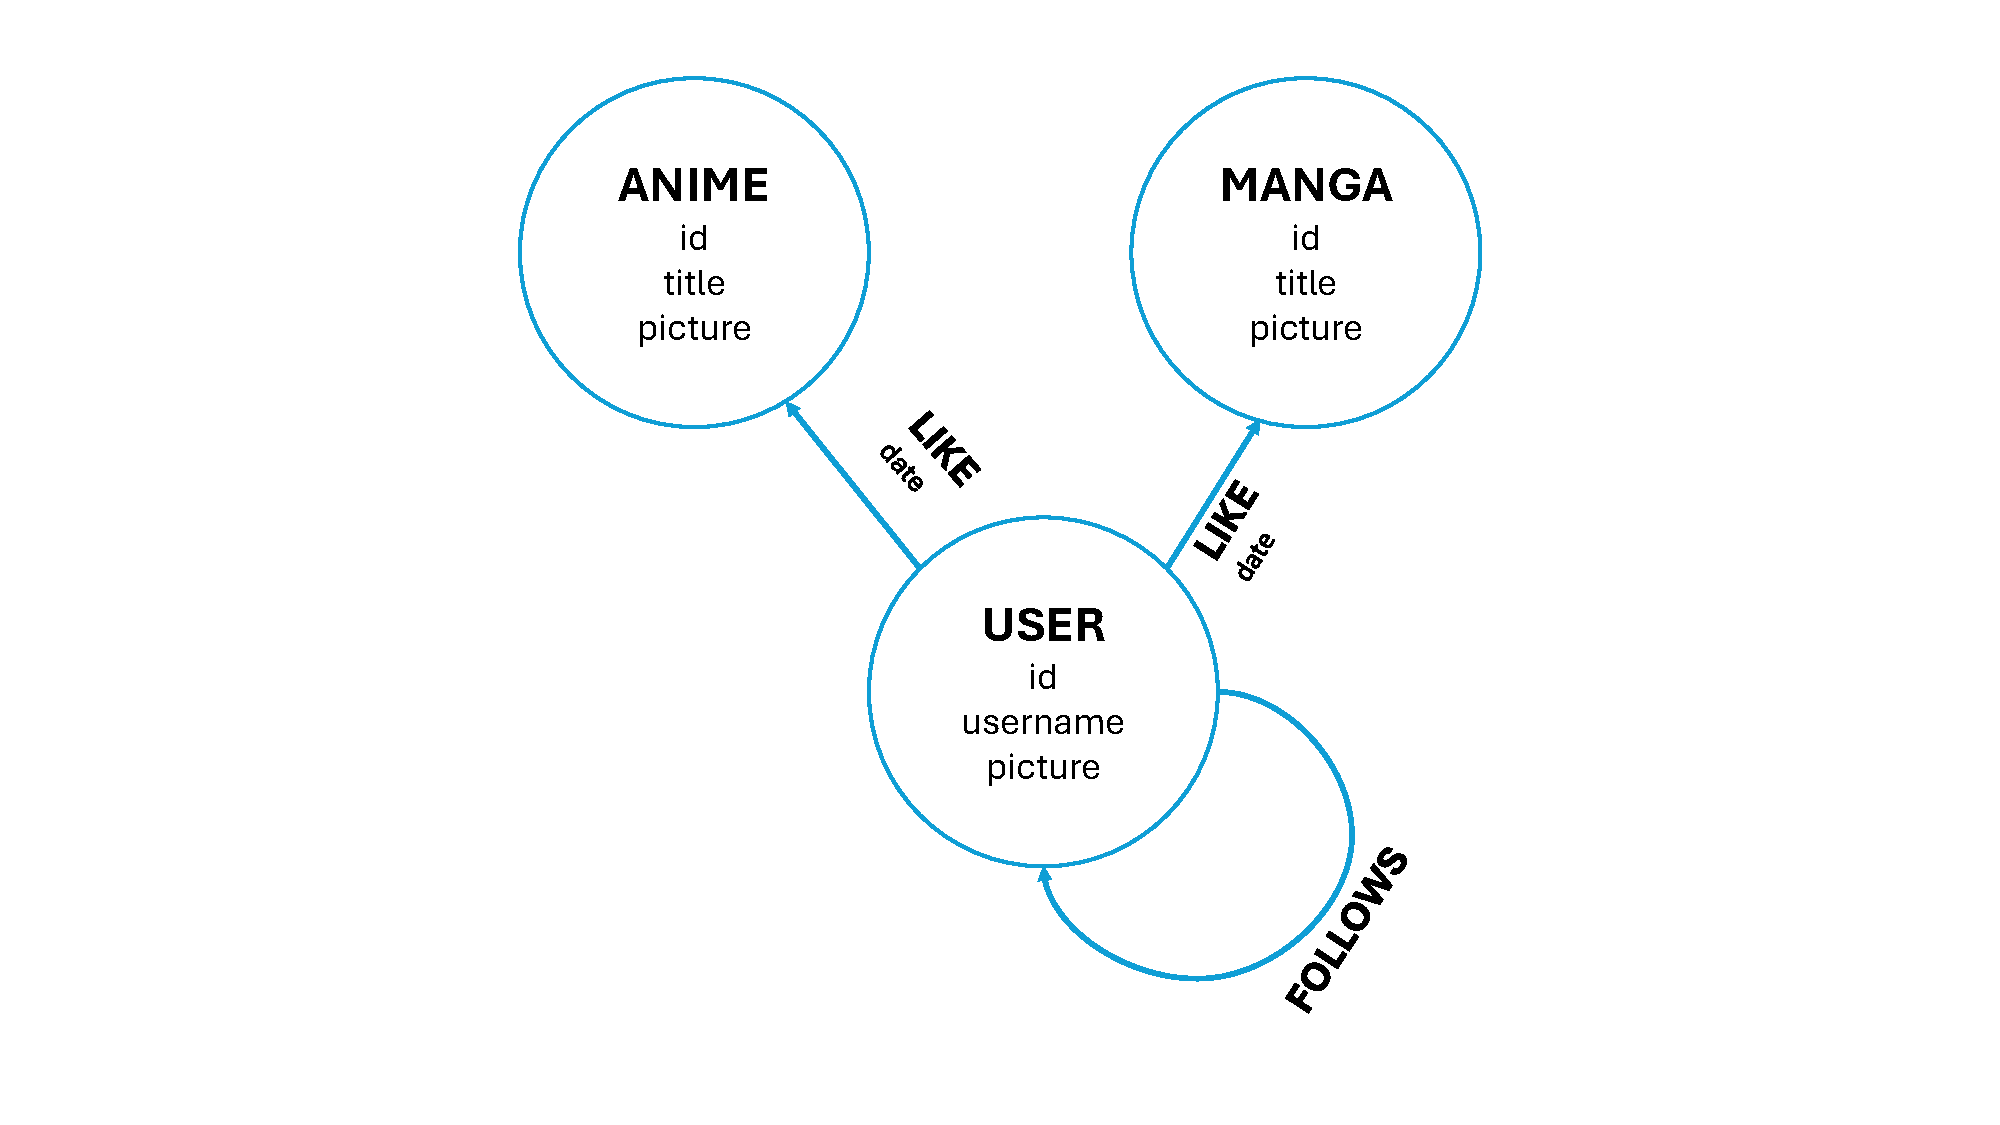
\includegraphics[width=\textwidth]{Media/graph.pdf}
    \caption{GraphDB}
    \label{fig:GraohDB}
\end{figure}

\newpage
\section{GraphDB queries}
Some of the most important Neo4j queries for analytic and suggestion porpouses.


\textbf{USERS:}

\begin{itemize}
  \item Suggest other users followings in common:
\end{itemize}
\begin{lstlisting}[language=Cypher, caption=SuggestUsersByCommonFollowings]

MATCH (u:User {id: $userId})-[:FOLLOWS]->(following:User)<-[:FOLLOWS]-(suggested:User) 
WHERE NOT (u)-[:FOLLOWS]->(suggested) AND u <> suggested 
WITH suggested, COUNT(DISTINCT following) AS commonFollowers 
WHERE commonFollowers > 5 
RETURN suggested as user, commonFollowers 
ORDER BY commonFollowers DESC 
LIMIT $n
\end{lstlisting}

\begin{itemize}
  \item Suggest other users likes in common:
\end{itemize}
\begin{lstlisting}[language=Cypher, caption=SuggestUsersByCommonLikes]
  MATCH (u:User {id: $userId})-[r:LIKE]->(media:Manga)<-[:LIKE]-(suggested:User) 
  WHERE u <> suggested AND r.date >= $date
  WITH suggested, COUNT(DISTINCT media) AS commonLikes
  WHERE commonLikes > $min
  RETURN suggested AS user, commonLikes
  ORDER BY commonLikes DESC
  LIMIT $n
\end{lstlisting}



\textbf{ANIME/MANGA:}

\begin{itemize}
  \item Suggest anime and manga based on following in common:
\end{itemize}
\begin{lstlisting}[language=Cypher, caption=GetSuggestedByFollowings]
  MATCH (u:User {id: $userId})-[:FOLLOWS]->(f:User)-[r:LIKE]->(a:Anime)
  WHERE NOT (u)-[:LIKE]->(a) AND r.date >= $startDate
  WITH a, COUNT(DISTINCT f) AS num_likes
  RETURN a AS anime
  ORDER BY num_likes DESC
  LIMIT $n
  
\end{lstlisting}


\begin{itemize}
  \item Suggest anime and manga based on likes in common between followers:
\end{itemize}
\begin{lstlisting}[language=Cypher, caption=GetSuggestedByLikes]
  MATCH (u:User {id: $userId})-[r1:LIKE]->(a:Anime)<-[:LIKE]-(f:User)
  WHERE r1.date >= $startDate
  WITH u, f, COUNT(a) AS common_likes
  ORDER BY common_likes DESC
  LIMIT 20
  MATCH (f)-[:LIKE]->(a2:Anime)
  WHERE NOT (u)-[:LIKE]->(a2)
  WITH a2, COUNT(DISTINCT f) AS num_likes
  RETURN a2 AS anime
  ORDER BY num_likes DESC
  LIMIT $n
  
\end{lstlisting}


\begin{itemize}
  \item Get the trend of media contents in a specific year based on the number of likes:
\end{itemize}
\begin{lstlisting}[language=Cypher, caption=GetTrendMediaContentByYear]
  MATCH (a:Anime)<-[r:LIKE]-(u:User)
  WHERE r.date >= $startDate AND r.date < $endDate
  WITH a, count(r) AS numLikes
  ORDER BY numLikes DESC
  RETURN a AS anime, numLikes
  LIMIT $n
  
\end{lstlisting}

\begin{itemize}
  \item Get the general trend of media contents based on the number of likes:
\end{itemize}
\begin{lstlisting}[language=Cypher, caption=GetMediaContentTrendByLikes]
  MATCH (u:User)-[r:LIKE]->(a:Anime)
  WHERE r.date >= $startDate
  WITH a, COUNT(r) AS numLikes
  ORDER BY numLikes DESC
  RETURN a AS anime, numLikes
  LIMIT $n
  
\end{lstlisting}


\subsection{CRUD operations}
\begin{itemize}
    \item Create: This operation will allow users to create new nodes and relationships in the database. For example, users can create new relationships between users and media content:
    
    An user can LIKE a media content: 
    \begin{lstlisting}[language=Cypher, caption=Create Like Relationship]
    MATCH (u:User {id: $userId}), (a:Anime {id: $animeId}) 
    WHERE NOT (u)-[:LIKE]->(a) 
    CREATE (u)-[r:LIKE {date: $date} ]->(a)
    RETURN r
    \end{lstlisting}

    A user can FOLLOW another user:
    \begin{lstlisting}[language=Cypher, caption=Create Follow Relationship]
    MATCH (u:User {id: $userId}), (f:User {id: $followedUserId}) 
    WHERE NOT (u)-[:FOLLOWS]->(f) 
    CREATE (u)-[r:FOLLOWS]->(f) 
    RETURN r
    \end{lstlisting}

    \item Read: This operation will allow users to read nodes and relationships from the database. For example, users can read information about anime and manga and relationships between users and media content.
    An user can read the list of liked media contents:
    \begin{lstlisting}[language=Cypher, caption=Read Liked Media Contents]
  
    MATCH (u:User {id: $userId})-[:LIKE]->(a:Anime)
    RETURN a
    \end{lstlisting}

    An user can read the list of followers:
    \begin{lstlisting}[language=Cypher, caption=Read Followers]
    MATCH (u:User {id: $userId})<-[:FOLLOWS]-(f:User)
    RETURN f
    \end{lstlisting}
  
    \item Update: This operation will allow users to update nodes and relationships in the database. For example, users can update their likes for anime and manga and relationships between users.
    
    \item Delete: This operation will allow users to delete nodes and relationships from the database. For example, users can delete their likes for anime and manga and relationships between users.
    
    An user can unlike a media content:
    \begin{lstlisting}[language=Cypher, caption=Delete Like Relationship]
    MATCH (u:User {id: $userId})-[r:LIKE]->(a:Anime {id: $animeId})
    DELETE r
    RETURN r
    \end{lstlisting}
    \newpage
    An user can unfollow another user: 
    \begin{lstlisting}[language=Cypher, caption=Delete Follow Relationship]
    MATCH (:User {id: $followerUserId})-[r:FOLLOWS]->(:User {id: $followingUserId})
    DELETE r 
    RETURN r
    \end{lstlisting}
\end{itemize}

\section{Redundancy}
The performance of the application is critical, so we need to ensure that the system is highly available and fault-tolerant. To achieve this, we gave priority to fast responses, rather than reducing memory consumption.


\textbf{Latest reviews}


In the anime and manga collections, there's a field containing the latest 5 reviews written for that specific media content, in this way it's fast to retrieve. 


\textbf{Average rating}


In the anime and manga collections, there's a field containing the average rating of the media content, this field is updated every time a new review is written.


\textbf{Number of likes}


In the anime and manga collections, there's a field containing the number of likes, this field is updated every time a new like relationship is created or deleted.


\textbf{Followers and Followings}


In the user collection, there are fields containing the number of followers and followings, this field is updated every time a new follow relationship is created or deleted.


\textbf{User field in Reviews}


In the reviews collection, there's a field containing the user data, such as id, username, picture, and also location and birthday, which are used for suggestion porpouses.

\section{Replicas}
The performance of the application is critical, so we need to ensure that the system is highly available and fault-tolerant. To achieve this, we will use a replication strategy for both the document and graph databases. This will allow us to have multiple copies of the data, so if one server fails, the system can continue to operate without any downtime.



\chapter{Implementation}

\section{Development Environment}
To ensure efficient and successful Implementation of MangaVerse web application,
choosing the appropriate development environment is one of the most important points of the project.

\subsection*{Programming Languages}
\begin{itemize}
    \item \textbf{Backend:} Java is the main programming language used in the project’s backend development.
    \item \textbf{Frontend:} HTML, CSS, JavaScript are utilized for building user interface in the project.
    \item \textbf{Data Preprocessing:} Python and java were used in the project to conduct data preprocessing task with the help of its powerful libraries and ease of use features. 
\end{itemize}

\subsection*{Database}
\begin{itemize}
    \item \textbf{Document Database:} MongoDB is used in the project to store and manage document-based data with the help of its flexibility and scalability features.
    \item \textbf{Graph Database:} Neo4j is used in the project to manage and query graph data and handle complex relationships and connections between user entities and media contents in an efficient way.
\end{itemize}

\subsection*{Integrated Development Environment} Intellij IDEA was used as an primary IDE. It is powerful Java 
integrated development environment for developing software in an efficient way.

\subsection*{Version Control} Github was used to provide a collaborative development with its version control system.

\subsection*{Web Server} Apache Tomcat was used as a web server to provide reliable environment for deploying and running the java based web application.

\subsection*{Build Automation} Maven was used as a build automation tool. It is used to manage the project's build, reporting, and documentation from a central piece of information.

\subsection*{Testing} JUnit was used as a testing framework for Java code. It is used to write and run repeatable automated tests. This ensures the reliability and efficiency of the codebase throughout the development process.





\section{Main Modules}
\begin{itemize}
    \item Configuration
    \item Controller
    \item DAO (Data Access Objects)
    \item DTO (Data Transfer Objects)
    \item Model 
    \item Service
    \item Utils
    \item User Interface
\end{itemize}
\subsection*{Configuration}
Configuration module contains a class named \textit{AppServletContextListener} which is responsible for 
initializing and managing database connections for the web application. The configuration class 
implements ServletContextListener interface. \textit{@WebListener} annotation is used to provide listening for 
application lifecycle events. This annotation contains two methods, which are \textit{contextInitialized(ServletContextEvent sce)} and
\textit{contextDestroyed(ServletContextEvent sce)}. The first method is called when the web application is started and the second method is called when the web application is shut down.\\ \\
\textbf{Database Connection Management:} Database connection is provided with \textit{openConnection()} and \textit{closeConnection()} methods. They are both initialized for managing connection
for MongoDB and Neo4j databases. Connections are managed with corresponding DAO classes which are BaseMongoDBDAO and BaseNeo4jDAO.\\ \\
With using the configuration module for database connection, web application ensures robustness and reliability in its data access layer.

\subsection*{Controller}
%%TODO: change the code when it is corrected 
The controller modules plays a role as intermediary between the user requests and backend of the MangaVerse wab application as servlet classes.
They receives the user requests, process them and returns with the corresponding response. The controller classes are implemented using HttpServlet to handle user requests and responses.
Within the scope of their intermediary role, the controller classes are responsible of being a bridge between the user interface and backend logic. 
When a user interacts with the web application, their actions are translated into a HTTP request and these requests are handled by the related servlet class in the controller module. 
To be able to do do request translation in an efficient way each controller class extend 'HttpServlet' and has various methods to handle HTTP requests like GET and POST. 
Each controller class utilized a switch-case structure to determine the action requested and invokes the appropriate handler method accordingly.
This structure allows for clear and organized routing of request to their corresponding handler method. After processing the request, the servlet generates a requested response.\\
\newline
\textbf{Example code snippet from MediaContentServlet:}
\begin{mdframed}[backgroundcolor=yellow!20, innerleftmargin=10pt, innerrightmargin=10pt]
    \begin{lstlisting}[language=java]
{
    protected void processRequest(HttpServletRequest request, HttpServletResponse response) throws ServletException, IOException {
        String action = request.getParameter("action");

        switch (action) {
            case "toggleLike" -> handleToggleLike(request, response);
            case "addReview" -> handleAddReview(request, response);
            case "deleteReview" -> handleDeleteReview(request, response);
            case "editReview" -> handleEditReview(request, response);
            case "getMediaContent" -> handleGetMediaContentById(request,response);
            case "getMediaContentByTitle" -> handleSearchMediaContentByTitle(request,response);
            case null, default -> handleLoadPage(request,response);
        }
    }
}
    \end{lstlisting}
\end{mdframed}
The controller module contains the following classes:
\begin{itemize}
    \item Exception \\
    NotAuthorizedException: This exception is thrown when the user is not authorized to access the requested resource.
    \item AuthServlet \\
    The AuthServlet class handles the user authentication and authorization processes. It includes login, logout and sign up functions
    \item MainPageServlet \\
    The MainPageServlet class is responsible for handling the main page of the web application. It includes the main page of the web application and the search functionality.
    It provides request related to displaying main page and searching media contents.
    \item ManagerServlet \\
    The ManagerServlet class manages administrative requests in manager page. These request are primarily about manga, anime and user analytics such \textit{averageRatingByMonth(), trendMediaContentByYear(), getBestCriteria()...}
    \item MediaContentServlet \\
    The MediaContentServlet class is responsible for managing request related with media contents. These requests include like, adding,deleting or editing reviews and retrieving media content details. 
    \item ProfileServlet \\
    The ProfileServlet class is responsible for managing user profile related requests. These requests include updating user profile, following/unfollowing other users, getting user profile details such as liked anime and manga and user reviews.
    \item UserServlet \\
    The UserServlet class is responsible for managing user related requests and interactions. These requests include retrieving followers list, following list and user information. 
\end{itemize}

\subsection*{DAO (Data Access Objects)}
The DAO module includes the logic for accessing and managing data in the database and provides data retrieval, 
storage and manipulation. This module includes classes with CRUD (create, read, update, delete) operations and query executions. 
It provides a layer of abstraction between the database and the rest of the application and ensures the separation of concerns. The DAO module contains the following classes:
\begin{itemize}
    \item Enums \\
    - DataRepositoryEnum
    \item Exceptions 
    \item Interfaces \\
    - MedıaContentDAO \\
    - ReviewDAO \\
    - UserDAO 
    \item Mongo \\
    - AnimeDAOMongoImpl \\
    - BaseMongoDBDAO \\
    - MangaDAOMongoImpl \\
    - ReviewDAOMongoImpl \\
    - UserDAOMongoImpl 
    \item Neo4j \\
    - AnimeDAONeo4jImpl \\
    - BaseNeo4jDAO \\
    - MangaDAONeo4jImpl \\
    - UserDAONeo4jImpl 
    \item DAOLocator 
\end{itemize}
\newpage
\textbf{Example code snippet from MangaDAOMongoImpl:}
\begin{mdframed}[backgroundcolor=yellow!20, innerleftmargin=10pt, innerrightmargin=10pt]
    \begin{lstlisting}[language=java]
{
    //MongoDB queries
    //Best genres/themes/demographics/authors based on the average rating
    @Override
    public Map<String, Double> getBestCriteria (String criteria, boolean isArray, int page) throws DAOException {
        try  {
            MongoCollection<Document> mangaCollection = getCollection(COLLECTION_NAME);
            int pageOffset = (page-1)*Constants.PAGE_SIZE;

            List<Bson> pipeline;
            if (isArray) {
                pipeline = List.of(
                        match(and(exists(criteria), ne("average_rating", null))),
                        unwind("$" + criteria),
                        group("$" + criteria, avg("criteria_average_rating", "$average_rating")),
                        sort(descending("criteria_average_rating")),
                        skip(pageOffset),
                        limit(25)
                );
            } else {
                pipeline = List.of(
                        match(Filters.exists(criteria)),
                        group("$" + criteria, avg("criteria_average_rating", "$average_rating")),
                        sort(new Document("criteria_average_rating", -1)),
                        skip(pageOffset),
                        limit(25)
                );
            }

            List <Document> document = mangaCollection.aggregate(pipeline).into(new ArrayList<>());
            Map<String, Double> bestCriteria = new LinkedHashMap<>();
            for (Document doc : document) {
                Double avgRating = doc.get("criteria_average_rating") instanceof Integer?
                        doc.getInteger("criteria_average_rating").doubleValue() :
                        doc.getDouble("criteria_average_rating");
                if (criteria.equals("authors")) {
                    bestCriteria.put(doc.get("_id", Document.class).getString("name"), avgRating);
                } else {
                    bestCriteria.put(doc.get("_id").toString(), avgRating);
                }
            }

            return bestCriteria;

        } catch (Exception e) {
            throw new DAOException(DAOExceptionType.GENERIC_ERROR, e.getMessage());
        }
    }
}
    \end{lstlisting}
\end{mdframed}


\newpage
\textbf{Example code snippet from UserDAONeo4jImpl:}
\begin{mdframed}[backgroundcolor=yellow!20, innerleftmargin=10pt, innerrightmargin=10pt]
    \begin{lstlisting}[language=java]
{
    /**
    * Retrieves a list of users following a specific user from the Neo4j database.
    *
    * @param userId The ID of the user whose followers are to be retrieved.
    * @param loggedUserId The ID of the user requesting the list of followers.
    * @return A list of RegisteredUserDTO objects representing the followers of the specified user.
    * @throws DAOException If an error occurs while retrieving the followers list.
    */
   @Override
   public List<UserSummaryDTO> getFirstNFollowers(String userId, String loggedUserId) throws DAOException {
       try (Session session = getSession()) {
           StringBuilder queryBuilder = new StringBuilder("MATCH (follower:User)-[:FOLLOWS]->(:User {id: $userId}) ");
           if (loggedUserId != null) {
               queryBuilder.append("WHERE follower.id <> $loggedUserId ");
           }
           queryBuilder.append("RETURN follower AS user ");
           queryBuilder.append("ORDER BY follower.username ");
           queryBuilder.append("LIMIT 10");
           String query = queryBuilder.toString();

           Map<String, Object> params = new HashMap<>();
           params.put("userId", userId);
           if (loggedUserId != null) {
               params.put("loggedUserId", loggedUserId);
           }

           List<Record> records = session.executeRead(
                   tx -> tx.run(query, params).list()
           );

           return records.isEmpty() ? null : records.stream()
                   .map(this::recordToUserSummaryDTO)
                   .toList();

       } catch (Neo4jException e) {
           throw new DAOException(DAOExceptionType.DATABASE_ERROR, e.getMessage());

       } catch (Exception e) {
           throw new DAOException(DAOExceptionType.GENERIC_ERROR, e.getMessage());
       }
   }
}
    \end{lstlisting}
\end{mdframed}
\newpage


\subsection*{DTO (Data Transfer Objects)}
The DTO modules are the intermediary class between presentation layer and the DAO module in the web application.
They transfer data structures between different layers and components of the application in a more standardized way.


\subsection*{Model}
\begin{itemize}
    \item Enums
    \item Media Content \\
    - Anime\\
    - Manga \\
    - Manga Author \\
    - Media Content
    \item Registered User\\
    - Mangager\\
    - Registered User\\
    - User
    \item Review 
\end{itemize}

\subsection*{Service}
Service module has also important role in the web application. The classes in the service module are responsible for containing
the business logic and maintaining interaction between the DAO classes and the presentation layer. 
It handles complex operations with guarantying that the application's core functionalities are executed correctly. Some of the services
that are provided in the service module are: \textit{UserService, MediaContentService, ReviewService, TaskManager, ExecuterTaskService}. The 
package structure of Service module is as follows:





\begin{itemize}
    \item enums \\
    - ExecuterTaskService
    \item exceptions \\
    - enums \\
    ----- BusinessExceptionType \\
    - BusinessException
    \item impl \\
    - asinc media tasks\\
    ----- CreateMediaTask\\
    ----- DeleteMediaTask\\
    ----- UpdateAverageRatingTask\\
    ----- UpdateMediaRedundancyTask\\
    ----- UpdateMediaTask\\
    ----- UpdateNumberofLikesTask\\
    - asinc review tasks\\
    ----- RemoveDeletedMediaReviewsTask\\
    ----- RemoveDeletedUserReviewsTask\\
    ----- UpdateReviewRedundancyTask\\
    - asinc user tasks\\
    ----- CreateUserTask\\
    ----- DeleteUserTask\\
    ----- UpdateNumberOfFollowedTask\\
    ----- UpdateNumberOfFollowersTask\\
    ---- UpdateUserTask\\
    - AperiodicExecutorTaskServiceImpl\\
    - ErrorTaskManager\\
    - MediaContentServiceImpl\\
    - PeriodicExecutorTaskServiceImpl\\
    - ReviewServiceImpl\\
    - UserServiceImpl\\
    - interfaces \\
    ----- ExecuterTaskService\\
    ----- MediaContentService\\
    ----- ReviewService\\
    ----- Task\\
    ----- TaskManager\\
    ----- UserService
    \item ServiceLocator
\end{itemize}

\section{Adopted Patterns and Techniques}
\subsection*{Patterns}


\subsection*{Techniques}

\textbf{Task Manager:}\\
Task Manager class which is located in the service module of the system provides asynchronous task execution with using 
\textit{PriorityBlockingQueue}. It helps to order the tasks according to their prioritizes. 
After that prioritization, it ensures that higher priority tasks will be executed first and if two tasks have the 
same priority the one which is created before will be executed first. While Task Manager class is able to start and stop the tasks within the functions inside,
it can also take tasks to the queue in a thread-safe way. By using taskComparator for ordering the tasks,
the system provides also effective scheduling and execution. \\ \\
\textbf{Aperiodic Executor Task Service:}\\
Executor Task Service class which is located inside the service module of the system is an important part for providing the eventual consistency. Executing tasks in asynchronous way with threads guarantees
eventual consistency across different collections, mongoDB and neo4j and different replicas. 
With the help of the Executor Task Service, tasks that are needed to be executed in an asynchronous way are handled by ensuring that changes propagate correctly across different part of the system.
While using multiple databases and data replicas for this web application, it is important for maintain data integrity and eventual consistency.
Executing the tasks in an asynchronous way using threads allows to perform operations without blocking the main execution flow.
Aperiodic executer task service class is implemented by using the interface of executor service. 


\section{Description of Main Classes}

\subsection*{Controller}
\renewcommand{\arraystretch}{1.5}
\begin{longtable}{|>{\arraybackslash}p{0.33\linewidth}|>{\arraybackslash}p{0.66\linewidth}|}
    \hline
    \textbf{Class} & \textbf{Description} \\
    \hline
    \endfirsthead

    \hline
    \textbf{Class} & \textbf{Description} \\
    \hline
    \endhead

    \hline
    \endfoot

    \hline
    \endlastfoot

    AuthServlet & Handles business logic for authentication \\
    \hline
    MainPageServlet & Handles business logic for main page \\
    \hline
    ManagerServlet & Handles business logic for manager \\
    \hline
    MediaContentServlet & Handles business logic for media content \\
    \hline
    ProfileServlet & Handles business logic for profile \\
    \hline
    UserServlet & Handles business logic for user \\
    \hline
\end{longtable}

\newpage

\subsection*{DAO}
\renewcommand{\arraystretch}{1.5}
\begin{longtable}{|>{\raggedright\arraybackslash}p{0.3\linewidth}|>{\raggedright\arraybackslash}p{0.1\linewidth}|>{\raggedright\arraybackslash}p{0.6\linewidth}|}
    \hline
    \textbf{Class} & \textbf{Sub-package} & \textbf{Description} \\
    \hline
    \endfirsthead

    \hline
    \textbf{Class} & \textbf{Sub-package} & \textbf{Description} \\
    \hline
    \endhead

    \hline
    \endfoot

    \hline
    \endlastfoot

    MediaContentDAO & interfaces & Collection of methods for media content database related entities on mongoDB \\
    \hline
    ReviewDAO B & interfaces & Collection of methods for review database related entities on mongoDB \\
    \hline
    UserDAO & interfaces & Collection of methods for user database related entities on mongoDB \\
    \hline
    AnimeDAOMongoImpl & mongo & Contains all the method implementation for the MongoDB database anime entities \\
    \hline      
    BaseMongoDBDAO & mongo & Contains all the method implementations for the MongoDB database \\
    \hline
    MangaDAOMongoImpl & mongo & Contains all the method implementations for the MongoDB database manga entities \\
    \hline
    ReviewDAOMongoImpl & mongo & Contains all the method implementations for the MongoDB database review entities \\
    \hline
    UserDAOMongoImpl & mongo & Contains all the method implementations for the MongoDB database user entities \\
    \hline
    AnimeDAONeo4jImpl & neo4j & Contains all the method implementation for the Neo4j database anime entities \\
    \hline
    BaseNeo4jDAO & neo4j & Contains all the method implementations for the Neo4j database \\
    \hline
    MangaDAONeo4jImpl & neo4j & Contains all the method implementation for the Neo4j database manga entities \\
    \hline
    UserDAONeo4jImpl & neo4j & Contains all the method implementation for the Neo4j database user entities \\
    \hline
    DAOLocator & & Implements the locator pattern for accessing DAOs based on the specified data repository \\
    \hline
\end{longtable}

\subsection*{DTO}
\renewcommand{\arraystretch}{1.5}
\begin{longtable}{|>{\raggedright\arraybackslash}p{0.25\linewidth}|>{\raggedright\arraybackslash}p{0.15\linewidth}|>{\raggedright\arraybackslash}p{0.6\linewidth}|}
    \hline
    \textbf{Class} & \textbf{Sub-package} & \textbf{Description} \\
    \hline
    \endfirsthead

    \hline
    \textbf{Class} & \textbf{Sub-package} & \textbf{Description} \\
    \hline
    \endhead

    \hline
    \endfoot

    \hline
    \endlastfoot

    AnimeDTO & mediaContent & Represents data transfer object containing attributes for animes \\
    \hline
    MangaDTO & mediaContent & Represents data transfer object containing attributes for mangas \\
    \hline
    MediaContentDTO & interfaces & Defines common attributes for media content \\
    \hline
    DashboardDTO & statistics & Contains statistical data for the dashboard \\
    \hline
    MongoDBStats & statistics & Provides statistics specific to MongoDB \\
    \hline
    LoggedUserDTO & & Holds information about a logged-in user. \\
    \hline
    PageDTO & & Represents pagination details \\
    \hline
    ReviewDTO & & Contains attributes for reviews \\
    \hline
    UserRegistrationDTO & & Holds data for user registration \\
    \hline
    UserSummaryDTO & & Provides a summary of user information \\
    \hline
\end{longtable}


\subsection*{Model}
\renewcommand{\arraystretch}{1.5}
\begin{longtable}{|>{\raggedright\arraybackslash}p{0.25\linewidth}|>{\raggedright\arraybackslash}p{0.15\linewidth}|>{\raggedright\arraybackslash}p{0.6\linewidth}|}
    \hline
    \textbf{Class} & \textbf{Sub-package} & \textbf{Description} \\
    \hline
    \endfirsthead

    \hline
    \textbf{Class} & \textbf{Sub-package} & \textbf{Description} \\
    \hline
    \endhead

    \hline
    \endfoot

    \hline
    \endlastfoot

    Anime & mediaContent & Provides unique anime attributes by extending parent class MediaContent and related getter and setter methods. \\
    \hline
    Manga & mediaContent & Provides unique manga attributes by extending parent class MediaContent and related getter and setter methods. \\
    \hline
    MangaAuthor & mediaContent & Contains manga author attributes and related getter and setter methods. \\
    \hline
    MediaContent & mediaContent & Contains all the attributes used by types of media contents and their getter and setter methods. \\
    \hline
    Manager & registeredUser & Provides unique manager attributes by extending parent class RegisteredUser and related getter and setter methods. \\
    \hline
    RegisteredUSer & registeredUser & Contains all the attributes used by types of registered users and their getter and setter methods. \\
    \hline
    User & registeredUser & Provides unique user attributes by extending parent class RegisteredUser and related getter and setter methods. \\
    \hline
    Review &  & Contains review attributes and related getter and setter methods. \\
    \hline
\end{longtable}



\subsection*{Service}
\renewcommand{\arraystretch}{1.5} % Adjusts the row height
\begin{longtable}{|>{\raggedright\arraybackslash}p{0.3\linewidth}|>{\raggedright\arraybackslash}p{0.2\linewidth}|>{\raggedright\arraybackslash}p{0.5\linewidth}|}
   
    \hline
    \textbf{Class} & \textbf{Sub-package} & \textbf{Description} \\
    \hline
    \endfirsthead

    \hline
    \textbf{Class} & \textbf{Sub-package} & \textbf{Description} \\
    \hline
    \endhead

    \hline
    \endfoot

    \hline
    \endlastfoot

    CreateMediaTask & impl/ asinc\_media\_tasks & Implementation of methods for media task creation for MediaContentService \\
    \hline
    DeleteMediaTask B & impl/ asinc\_media\_tasks & Implementation of methods for media task deletion for MediaContentService \\
    \hline
    RefreshLatestReviewsTasks & impl/ asinc\_media\_tasks & Implementation of methods for refreshing latest reviews for MediaContentService \\
    \hline
    UpdateAverageRatingTask & impl/ asinc\_media\_tasks & Implementation of methods for updating average rating for MediaContentService \\
    \hline
    UpdateMediaRedundancyTask & impl/ asinc\_media\_tasks & Implementation of methods for updating media redundancy for MediaContentService \\
    \hline
    UpdateMediaTask & impl/ asinc\_media\_tasks & Implementation of methods for updating media for MediaContentService \\
    \hline
    UpdateNumberofLikesTask & impl/ asinc\_media\_tasks & Implementation of methods for updating numbers of likes for MediaContentService \\
    \hline
    RemoveDeletedMedia ReviewsTask & impl/ asinc\_review\_tasks & Implementation of methods for removing reviews of deleted media for ReviewService \\
    \hline
    RemoveDeletedUser ReviewsTask & impl/ asinc\_review\_tasks & Implementation of methods for removing reviews of deleted user for ReviewService \\
    \hline
    UpdateReviewRedundancyTask & impl/ asinc\_review\_tasks & Implementation of methods for updating review redundancy for ReviewService \\
    \hline
    CreateUserTask & impl/ asinc\_user\_tasks & Implementation of methods for user creation for UserService \\
    \hline
    DeleteUserTask & impl/ asinc\_user\_tasks & Implementation of methods for user deletion for UserService \\
    \hline
    UpdateNumberOfFollowedTask B & impl/ asinc\_user\_tasks & Implementation of methods for updating number of followed for UserService \\
    \hline
    UpdateNumberOfFollowersTask & impl/ asinc\_user\_tasks & Implementation of methods for updating number of followers for UserService \\
    \hline
    UpdateUserTask & impl/ asinc\_user\_tasks & Implementation of methods for updating user for MediaContentService \\
    \hline
    AperiodicExecutor TaskServiceImpl & impl & Implementation of aperiodic tasks for ExecutorTaskService \\
    \hline
    ErrorTaskManager & impl & Implementation of TaskManager interface to handle error \\
    \hline
    MediaContentServiceImpl & impl & Implementation of MediaContentService, providing media content operations \\
    \hline
    PeriodicExecutor TaskServiceImpl & impl & Implementation of periodic tasks for ExecutorTaskService \\
    \hline
    ReviewServiceImpl & impl & Implementation of ReviewService, providing review operations \\
    \hline
    UserServiceImpl & impl & Implementation of UserService, providing user operations \\
    \hline
    ExecutorTaskService & interfaces & Collection of methods for task management \\
    \hline
    MediaContentService & interfaces & Collection of methods for media content service \\
    \hline
    ReviewService & interfaces & Collection of methods for review service \\
    \hline
    Task & interfaces & Collection of methods for execution operations \\
    \hline
    TaskManager & interfaces & Collection of methods for managing task prioritization \\
    \hline
    UserService & interfaces & Collection of methods for user service \\
    \hline
    ServiceLocator & & Implements locator pattern for services \\
    \hline
\end{longtable}



\newpage
\section {MongoDB queries}
Some of the most important MongoDB queries for analytic and suggestion purposes. 
%% TODO: write the mongoshell query and the java implementation with explaination
%% suggestUserByCommonLikes, getDistribution, averageAppRating, averageAppRatingByAge, 
%% suggestUsersByCommonFollowings, getMediaContentRatingByYear, getMediaContentRatingByMonth,
%% suggestMediaContent, getBestCriteria, getTrendMediaContentByYear, getMediaContentTrendByLikes,
%% getSuggestedByFollowings, getSuggestedByLikes(suggest and trenda are on neo4j, sadece suggest media content mongo db, ona göre mongo ya da neo4j kısmına koy)

\textbf{USERS:}
\begin{itemize}
  \item GetDistribution query to get the user's location, gender, birthday year that gave the highest rating to the application:
  
\end{itemize}
\begin{lstlisting}[language=JavaScript, caption=GetDistribution]
  // Match stage to filter documents where 'criteriaOfSearch' exists
  db.collection.aggregate([
      {
          $match: {
              [criteriaOfSearch]: { $exists: true }
          }
      },
      // Project stage to include 'criteriaOfSearch' and 'app_rating' fields
      {
          $project: {
              [criteriaOfSearch]: 1,
              app_rating: 1
          }
      },
      // Group stage to count occurrences of each 'criteriaOfSearch'
      {
          $group: {
              _id: "$" + criteriaOfSearch,
              count: { $sum: 1 }
          }
      },
      // Sort stage to sort documents by 'count' in descending order
      {
          $sort: {
              count: -1
          }
      }
  ]);
  \end{lstlisting}
  


\textbf{ANIME/MANGA:}

\begin{itemize}

\item GetBestCriteria query, the criteria can be genres, demographics, themes, authors and serialization for manga; tags, producers, studios for anime:
\begin{lstlisting}[language=JavaScript, caption=GetBestCriteria]
  db.collection.aggregate([
      // Match stage to filter documents where 'criteria' exists and 'average_rating' is not null
      {
          $match: {
              criteria: { $exists: true },
              average_rating: { $ne: null }
          }
      },
      // Unwind stage to deconstruct the 'criteria' array field
      {
          $unwind: "$" + criteria
      },
      // Group stage to calculate the average rating for each criteria
      {
          $group: {
              _id: "$" + criteria,
              criteria_average_rating: { $avg: "$average_rating" }
          }
      },
      // Sort stage to sort documents by 'criteria_average_rating' in descending order
      {
          $sort: {
              criteria_average_rating: -1
          }
      },
      // Skip stage to skip the first 'pageOffset' documents
      {
          $skip: pageOffset
      },
      // Limit stage to limit the results to 25 documents
      {
          $limit: 25
      }
  ]);
  \end{lstlisting}

\end{itemize}

\textbf{REVIEWS:}

\begin{itemize}
\item GetMediaContentRatingByYear query to get the average rating of media content by year:
\end{itemize}


\begin{lstlisting}[language=JavaScript, caption=GetMediaContentRatingByYear]
  // Match stage to filter documents based on specified conditions
  db.collection.aggregate([
      {
          $match: {
              [`${nodeType}.id`]: new ObjectId(mediaContentId),
              rating: { $exists: true },
              date: { $gte: startDate, $lt: endDate }
          }
      },
      // Group stage to group documents by year and calculate the average rating
      {
          $group: {
              _id: { $year: "$date" },
              average_rating: { $avg: "$rating" }
          }
      },
      // Project stage to shape the output documents
      {
          $project: {
              _id: 0,
              year: "$_id",
              average_rating: 1
          }
      },
      // Sort stage to sort documents by year in ascending order
      {
          $sort: { year: 1 }
      }
  ]);
  \end{lstlisting}


\begin{itemize}
  \item SuggestMediaContent query to suggest media content based on common criteria, like birthday or location:
  
\end{itemize}

\begin{lstlisting}[language=JavaScript, caption=SuggestMediaContent]
  db.collection.aggregate([
  {
    // Match documents based on a dynamic user criteria
    $match: {
      ["user." + criteriaType]: criteriaValue
    }
  },
  {
    // Group documents by node type ID and calculate the first title and average rating
    $group: {
      _id: "$" + nodeType + ".id", // Group by the node type's ID
      title: { $first: "$" + nodeType + ".title" }, // Get the first title in the group
      average_rating: { $avg: "$rating" } // Calculate the average rating for the group
    }
  },
  {
    // Sort the grouped documents by average rating in descending order
    $sort: { average_rating: -1 }
  },
  {
    // Limit the number of results to the page size constant
    $limit: Constants.PAGE_SIZE
  }
]);
\end{lstlisting}

\section{GraphDB queries}
Some of the most important Neo4j queries for analytic and suggestion porpouses.

\textbf{USERS:}

\begin{itemize}
  \item Suggest other users followings in common:
\end{itemize}
\begin{lstlisting}[language=Cypher, caption=SuggestUsersByCommonFollowings]

MATCH (u:User {id: $userId})-[:FOLLOWS]->(following:User)<-[:FOLLOWS]-(suggested:User) 
WHERE NOT (u)-[:FOLLOWS]->(suggested) AND u <> suggested 
WITH suggested, COUNT(DISTINCT following) AS commonFollowers 
WHERE commonFollowers > 5 
RETURN suggested as user, commonFollowers 
ORDER BY commonFollowers DESC 
LIMIT $n
\end{lstlisting}

\begin{itemize}
  \item Suggest other users likes in common:
\end{itemize}
\begin{lstlisting}[language=Cypher, caption=SuggestUsersByCommonLikes]
  MATCH (u:User {id: $userId})-[r:LIKE]->(media:Manga)<-[:LIKE]-(suggested:User) 
  WHERE u <> suggested AND r.date >= $date
  WITH suggested, COUNT(DISTINCT media) AS commonLikes
  WHERE commonLikes > $min
  RETURN suggested AS user, commonLikes
  ORDER BY commonLikes DESC
  LIMIT $n
\end{lstlisting}



\textbf{ANIME/MANGA:}

\begin{itemize}
  \item Suggest anime and manga based on following in common:
\end{itemize}
\begin{lstlisting}[language=Cypher, caption=GetSuggestedByFollowings]
  MATCH (u:User {id: $userId})-[:FOLLOWS]->(f:User)-[r:LIKE]->(a:Anime)
  WHERE NOT (u)-[:LIKE]->(a) AND r.date >= $startDate
  WITH a, COUNT(DISTINCT f) AS num_likes
  RETURN a AS anime
  ORDER BY num_likes DESC
  LIMIT $n
  
\end{lstlisting}


\begin{itemize}
  \item Suggest anime and manga based on likes in common between followers:
\end{itemize}
\begin{lstlisting}[language=Cypher, caption=GetSuggestedByLikes]
  MATCH (u:User {id: $userId})-[r1:LIKE]->(a:Anime)<-[:LIKE]-(f:User)
  WHERE r1.date >= $startDate
  WITH u, f, COUNT(a) AS common_likes
  ORDER BY common_likes DESC
  LIMIT 20
  MATCH (f)-[:LIKE]->(a2:Anime)
  WHERE NOT (u)-[:LIKE]->(a2)
  WITH a2, COUNT(DISTINCT f) AS num_likes
  RETURN a2 AS anime
  ORDER BY num_likes DESC
  LIMIT $n
  
\end{lstlisting}


\begin{itemize}
  \item Get the trend of media contents in a specific year based on the number of likes:
\end{itemize}
\begin{lstlisting}[language=Cypher, caption=GetTrendMediaContentByYear]
  MATCH (a:Anime)<-[r:LIKE]-(u:User)
  WHERE r.date >= $startDate AND r.date < $endDate
  WITH a, count(r) AS numLikes
  ORDER BY numLikes DESC
  RETURN a AS anime, numLikes
  LIMIT $n
  
\end{lstlisting}

\begin{itemize}
  \item Get the general trend of media contents based on the number of likes:
\end{itemize}
\begin{lstlisting}[language=Cypher, caption=GetMediaContentTrendByLikes]
  MATCH (u:User)-[r:LIKE]->(a:Anime)
  WHERE r.date >= $startDate
  WITH a, COUNT(r) AS numLikes
  ORDER BY numLikes DESC
  RETURN a AS anime, numLikes
  LIMIT $n
  
\end{lstlisting}

\chapter{Conclusion}

\section{Conclusion 1}
% Inserisci qui il contenuto della prima conclusione.

\section{Conclusion 2}
% Inserisci qui il contenuto della seconda conclusione.

% Aggiungi altri paragrafi e sezioni se necessario


\end{document}

